\section{Notation and implementation details}
\label{app:notation}

\begin{table}[htbp]
\centering\small
\begin{tabular}{ll}
\toprule
Symbol & Meaning and units \\
\midrule
$i,c,z,t$ & Home, county, load zone, dispatch interval \\
$\Delta$ & Dispatch duration, 0.25 h \\
$L_{i,t},V_{i,t}$ & Household demand and PV output, kW \\
$\bar E_i,E_i$ & Rated and SOH-adjusted available capacity, kWh \\
$e_{i,t},e_i^{\min}$ & Stored energy and physical minimum, kWh \\
$R_{i,t}$ & Connected operating reserve target, kWh \\
$p^c_{i,t},p^d_{i,t}$ & Nonnegative charging/discharging power, kW \\
$m_{i,t},x_{i,t}$ & Connected import/export power, kW \\
$\lambda_{z,t}$ & Real-time settlement price, \$/kWh in accounting \\
$U_{i,t},B_i$ & Interval unserved energy and annual reliability budget, kWh \\
$\lambda_r$ & Shared reliability penalty, \$/kWh of delivered energy \\
$\hat N_{i,t}$ & Historical five-hour usable-energy need, kWh stored \\
$\hat p_h$ & Forecast county-risk timing proxy at planning step $h$ \\
$f_{c,t}$ & Recorded county customers-out fraction \\
$u_p,u_r$ & Learned power fraction and reserve multiplier \\
$\varepsilon$ & Cumulative-risk threshold in the planning horizon \\
\bottomrule
\end{tabular}
\caption{Notation used in the model and results. Stored-energy requirements account for discharge efficiency; delivered unserved energy is scored in kWh at the household.}
\end{table}

The three hardware presets are $(\bar E,\bar P^c,\bar P^d)=(25,11.4,11.4)$, $(50,11.4,11.4)$, and $(39.2,20,20)$ in kWh/kW/kW. The reference evaluation mix is 60\%, 20\%, and 20\%, respectively. Both efficiencies are 0.9486833. The physical minimum is 5\% of rated energy; operating percentage targets use available energy. State of health is fixed at one in the principal evaluation, and randomized during training. Homes are sampled with replacement from each metropolitan pool.

For the five-hour need, each historical sample sums positive demand net of PV over 20 intervals, divides by discharge efficiency, and is grouped by local-time slot. The 90th percentile pools the target slot and its two neighboring quarter-hour slots on either side. Only samples whose entire forward window ends before episode start are eligible. Tier requirements repeat the calculation at their respective durations. PV surplus does not reduce a later positive-demand requirement in this conservative statistic; it can charge the battery in actual replay.

The learned reserve mapping is
\begin{equation}
R_{i,t}=\operatorname{clip}\left(u_r\hat N_{i,t},\,0.1E_i,\,0.9E_i\right),\qquad 0\le u_r\le1.
\end{equation}
This is an action parameterization, not an exact translation of the optimization shortfall target $\hat N+e^{\min}$. In particular, outside the alert override its multiplier cannot request arbitrarily more than the historical usable-energy statistic. That restriction is part of the evaluated learned controller, and limits claims about other learned reserve designs. The alert override takes the maximum of this target and $0.9E_i$ for affected homes.

The power proposal is $u_p$ times the currently realizable aggregate charge or discharge envelope, according to its sign. The priority allocator respects each home's feasible envelope. If enforcing a raised target requires additional charging, actual aggregate power can differ from that proposal. The absolute gap receives a reward penalty of 0.01 dollars per kW before division by fleet size. This engineering penalty is separate from the unserved-energy multiplier. Communication dropout is sampled independently per interval/home and disables remote trading actions; autonomous local islanded service remains available.

\paragraph{Optimization reference.}
Each home uses 32 equally spaced energy states between its physical minimum and available capacity. The horizon is at most 96 quarter-hours and shrinks at episode end. The program replans every four intervals, using current measured energy snapped to the nearest grid state for planning. Actual dispatch subsequently passes through continuous physical clipping and mandatory target recovery. Its terminal value is energy times discharge efficiency times the mean forecast wholesale price over that planning horizon; this is distinct from the fixed terminal inventory value used to compare realized episode margins. The hold-near-90\% reference adds a 0.02 \$/kWh-hour penalty on its energy gap below 90\%, above a 20\% floor. It is a soft high-SOC preference rather than a hard 90\% minimum.

An operating-floor shortfall receives a large planning penalty, while the execution layer enforces the target to the extent physically reachable within the interval. Risk DP adds Equation~\eqref{eq:surrogate}; the threshold rule raises each future planning step's floor when cumulative timing-proxy mass through that step reaches $\varepsilon$. Neither anticipates future individual islanding. The oracle-onset variant substitutes realized county 1\% threshold onsets, rather than realized home failures. Oracle onset and market lookahead are two separate information references.

\section{Complete training and reproduction protocol}
\label{app:repro}

The frozen main grid contains 21 runs. Promise-window training uses $\lambda_r\in\{5,20\}$ and seeds 1--5. Full-outage-cost learned-reserve training uses $\lambda_r=1$ at seeds 0--1, $\lambda_r=5$ at seeds 0--2, and $\lambda_r=20$ at seeds 0--1. Fixed-reserve and physical-minimum-only learned trading ablations use $\lambda_r=5$ at seeds 0--1. All retain physical clipping and the same policy architecture. Thus the physical-minimum-only ablation is not an unconstrained battery simulator.

Each run uses 2,998,272 transitions, or 732 complete rollouts of 16 environments times 256 intervals. There are six PPO epochs and four minibatches per rollout, Adam epsilon $10^{-5}$, gradient-norm clipping 0.5, value-loss coefficient 0.5, and a linearly decaying learning rate from $3\times10^{-4}$. Discount, GAE, and policy-clipping parameters are 0.997, 0.95, and 0.2. Entropy coefficient is 0.005 for promise-cost runs and zero for full-cost runs. Observations and discounted returns have online running mean/variance normalization. Minibatch advantages are standardized. Gaussian samples are clipped into the environment's power/reserve action ranges; the log-probability objective uses the sampled Gaussian action. This clipped-action convention is a limitation of this implementation, not a newly proposed PPO estimator.

The reference run uses one ARM64 CPU workstation with 11 logical processors and 18 GiB memory, up to six concurrent training processes, and one PyTorch thread per run. No GPU is used. Per-run configuration and progress logs retain the exact library versions, transition counts, and training times. File locks serialize any overlapping requests for the same run; parallel scheduling changes wall time, not the per-run budget or seed.

Training samples Houston 2019--2023, fleet size uniformly from 50--200, hardware presets uniformly across the three types, per-home SOH uniformly from 0.85--1, and per-episode dropout probability uniformly from 0--0.1. Half of proposals start near county events above 1\%, with a random offset of up to three days. Every proposed interval overlapping a named training-year event holdout is rejected. A failed search raises an error rather than silently accepting a holdout overlap. Historical feature buffers after an event can contain its past observations; no additional 28-day feature embargo is imposed.

Storm tests dated before 2024 are event holdouts within the training-year range, not chronological deployment backtests: the controller also trains on other, later dates in 2019--2023. Houston 2025 and 2026 are the chronological tests that postdate the entire PPO training period. ``Causal'' in the data protocol refers to the decision-time information set, including the pre-Uri hazard fit/calibration, rather than to a claim that the PPO controller was trained before every named storm.

Among the ten promise-cost candidates, selection maximizes Houston 2024 annualized adjusted margin minus 20 dollars per kWh of annualized first-five-hour unserved energy. Ties use controller name. The frozen selection is \SelectedRun. Neither guarded outcomes nor test-year/event performance enter this rule. Both guarded and unguarded versions of every checkpoint are evaluated on each main dataset; the selected comparison does not hide the remaining runs.

The main evaluation has five regular-year/metro datasets: Houston 2024, 2025, and partial 2026; DFW 2024; and San Antonio 2024. Six additional datasets are event-only: Houston 2021, 2022, and 2023; DFW 2021 and 2022; and San Antonio 2021. The three 2024 regular datasets also include named events in their output files, but those rows are never used in annualized aggregates. A machine-readable manifest lists every expected window and controller across 473 result files, and verifies exact coverage.

Replay uses seed zero for fleet selection, hardware assignment, and the separately initialized outage/availability draws. The homes and outage realizations are common across controllers within a dataset/scenario. Regular windows start at the first target-year timestamp after the preceding-history prefix and partition the available period without overlap. The final partial interval is retained. All episodes start with 90\% available charge. Annualization divides complete per-home totals by observed hours and multiplies by 8,760, including for the leap year and partial 2026; these are standardized rates.

The paper's aggregated cash-tail statistics use complete 24-hour blocks anchored at each window start; partial blocks are excluded. Per-window diagnostic columns can include a final short block and are not averaged to obtain these aggregates. CVaR$_5$ averages the lowest 5\% of those daily cash margins under the released quantile convention. The worst seven-block sum can cross a reset boundary and is not a continuous-operation worst-week estimate. Per-home promise quantiles include only homes with a simulated episode, while unserved-energy quantiles include every sampled home. Bootstrap intervals use 2,000 paired regular-window resamples with seed zero, pool episode/failure counts in each resample, and omit reliability resamples with no episodes.

Code and processed artifacts carry protocol and source hashes. All reported replays use the final \texttt{reserve-minimum-v3} controller revision and the corrected full-cycle throughput-aging normalization. Preliminary outputs are archived separately. Corrections to the training information, reward, and physical execution required fresh PPO training; the later change to the independent optimization controller does not alter the learned training dynamics.

\begin{table}[htbp]
\centering\small
\begin{tabular}{lrrrr}
\toprule
Run & $\Delta$ margin & Promise (\%) & Mean SOC (\%) & Throughput \\
\midrule
pc\_lam20\_s1 & -93.4 & 96.3 & 98.7 & 1,106.4 \\
pc\_lam20\_s2 & -105.6 & 86.3 & 96.2 & 2,090.4 \\
pc\_lam20\_s3 & -81.3 & 89.8 & 89.7 & 2,797.2 \\
pc\_lam20\_s4 & -159.3 & 91.9 & 56.5 & 12,048.3 \\
pc\_lam20\_s5 & -200.0 & 31.1 & 10.9 & 1,084.3 \\
pc\_lam5\_s1 & -55.3 & 96.3 & 97.4 & 2,323.0 \\
pc\_lam5\_s2 & -88.2 & 85.9 & 93.7 & 4,197.8 \\
pc\_lam5\_s3 & -238.3 & 68.7 & 45.0 & 14,808.9 \\
pc\_lam5\_s4* & -26.1 & 96.3 & 93.6 & 3,566.0 \\
pc\_lam5\_s5 & -210.4 & 31.8 & 20.2 & 1,439.8 \\
\bottomrule
\end{tabular}

\caption{All ten promise-cost candidates on Houston 2024. Asterisk denotes the fixed validation selection. Margin difference is \$/home-year against fixed 20\%; throughput is charge plus discharge kWh/home-year. Promise and mean SOC are percentages. Names encode penalty and seed.}
\label{tab:promise-seeds}
\end{table}

\begin{table}[htbp]
\centering\small
\begin{tabular}{lrrrr}
\toprule
Run & $\Delta$ margin & Promise (\%) & Mean SOC (\%) & Throughput \\
\midrule
fixed\_lam5\_s0 & -100.3 & 94.7 & 65.4 & 2,502.2 \\
fixed\_lam5\_s1 & -86.3 & 96.3 & 97.0 & 754.6 \\
learned\_lam1\_s0 & -46.9 & 95.6 & 88.9 & 1,207.5 \\
learned\_lam1\_s1 & -89.9 & 90.2 & 92.6 & 4,377.0 \\
learned\_lam20\_s0 & -2.2 & 80.3 & 95.1 & 3,225.7 \\
learned\_lam20\_s1 & -83.8 & 96.3 & 98.4 & 1,298.9 \\
learned\_lam5\_s0 & -137.0 & 90.2 & 38.5 & 2,132.7 \\
learned\_lam5\_s1 & -72.8 & 96.3 & 97.8 & 2,089.0 \\
learned\_lam5\_s2 & -106.4 & 86.3 & 96.5 & 2,767.6 \\
none\_lam5\_s0 & -148.5 & 64.7 & 12.7 & 2,121.8 \\
none\_lam5\_s1 & -232.3 & 39.7 & 13.7 & 1,979.6 \\
\bottomrule
\end{tabular}

\caption{All eleven full-outage-cost and reserve-ablation runs, with the same units as Table~\ref{tab:promise-seeds}. ``None'' removes the operating reserve but retains physical battery limits. These runs do not participate in selecting the headline promise-cost candidate.}
\label{tab:other-seeds}
\end{table}
\FloatBarrier

\clearpage
\section{Additional economic and household outcomes}
\label{app:tails}
\begingroup
\setlength{\intextsep}{8pt}

\begin{table}[!htbp]
\centering\small
\begin{tabular}{lrrrr}
\toprule
Controller & Cash/yr & Adjusted/yr & Daily CVaR$_5$ & Worst 7 blocks \\
\midrule
Fixed 20\% & 493.0 & 475.3 & -0.47 & 1.30 \\
Fixed 50\% & 405.9 & 395.8 & -0.48 & 1.19 \\
Hold near 90\% & 373.9 & 371.0 & -0.79 & 0.56 \\
Storm rule & 482.0 & 465.2 & -0.91 & 0.83 \\
Historical tiers & 414.5 & 401.7 & -0.48 & 1.22 \\
Risk DP 5 & 467.7 & 449.9 & -0.55 & 1.11 \\
Threshold 0.1 & 505.2 & 485.6 & -0.61 & 1.32 \\
Selected PPO & 448.6 & 449.2 & -1.39 & -0.96 \\
PPO + override & 449.3 & 449.9 & -1.35 & -0.64 \\
\bottomrule
\end{tabular}

\caption{Houston 2024 gross outcomes, in dollars per home. Cash and adjusted margins are annualized; daily CVaR and worst seven-block values use complete 24-hour cash blocks (Appendix~\ref{app:repro}). Higher values are preferable. Aging charges are excluded.}
\label{tab:tails}
\end{table}

\begin{table}[!htbp]
\centering\small
\begin{tabular}{lrrr}
\toprule
Controller & Homes with outages & Promise $p_5$\% & Unserved $p_{95}$/yr \\
\midrule
Fixed 20\% & 100 & 33.3 & 577.4 \\
Fixed 50\% & 100 & 66.2 & 547.2 \\
Hold near 90\% & 100 & 66.7 & 526.6 \\
Storm rule & 100 & 42.7 & 547.7 \\
Historical tiers & 100 & 49.6 & 548.4 \\
Risk DP 5 & 100 & 59.9 & 559.2 \\
Threshold 0.1 & 100 & 50.0 & 566.3 \\
Selected PPO & 100 & 74.8 & 518.0 \\
PPO + override & 100 & 74.8 & 518.0 \\
\bottomrule
\end{tabular}

\caption{Houston 2024 household tails. Promise $p_5$ is the fifth percentile of household episode-success rates among homes with outages (higher is better). Unserved $p_{95}$ is the 95th percentile of annualized household unserved energy, kWh/home-year (lower is better). These empirical quantiles do not certify household risk budgets.}
\label{tab:households}
\end{table}

\begin{table}[!htbp]
\centering\small
\begin{tabular}{llrrrr}
\toprule
Season & Dispatch & Hours & $\Delta$ margin/wk & Promise\% & Episodes \\
\midrule
DJF & Fixed 20\% & 2,400 & +0.0 & 88.9 & 18 \\
DJF & Threshold 0.1 & 2,400 & +0.0 & 88.9 & 18 \\
DJF & Risk DP 5 & 2,400 & -0.3 & 100.0 & 18 \\
DJF & Selected PPO & 2,400 & -0.7 & 100.0 & 18 \\
DJF & PPO + override & 2,400 & -0.6 & 100.0 & 18 \\
MAM & Fixed 20\% & 2,016 & +0.0 & 83.1 & 219 \\
MAM & Threshold 0.1 & 2,016 & +0.4 & 88.1 & 219 \\
MAM & Risk DP 5 & 2,016 & -0.3 & 87.2 & 219 \\
MAM & Selected PPO & 2,016 & -2.0 & 93.2 & 219 \\
MAM & PPO + override & 2,016 & -2.0 & 93.2 & 219 \\
JJA & Fixed 20\% & 2,352 & +0.0 & 67.4 & 316 \\
JJA & Threshold 0.1 & 2,352 & +0.1 & 84.5 & 316 \\
JJA & Risk DP 5 & 2,352 & -0.9 & 96.8 & 316 \\
JJA & Selected PPO & 2,352 & -0.4 & 98.1 & 316 \\
JJA & PPO + override & 2,352 & -0.4 & 98.1 & 316 \\
SON & Fixed 20\% & 2,016 & +0.0 & 100.0 & 16 \\
SON & Threshold 0.1 & 2,016 & +0.3 & 100.0 & 16 \\
SON & Risk DP 5 & 2,016 & -0.5 & 100.0 & 16 \\
SON & Selected PPO & 2,016 & +1.1 & 100.0 & 16 \\
SON & PPO + override & 2,016 & +1.1 & 100.0 & 16 \\
\bottomrule
\end{tabular}

\caption{Houston 2024 seasonal window cohorts, assigned by first local timestamp: DJF (Dec--Feb), MAM (Mar--May), JJA (Jun--Aug), and SON (Sep--Nov). Boundary-crossing windows remain whole; these are not exact calendar-season totals. Hours and episodes are observed; margin is standardized \$/home-week against fixed 20\%. Higher margin/promise is better. The released CSV retains all controllers/datasets and paired window-bootstrap intervals.}
\label{tab:seasonal}
\end{table}
\FloatBarrier
\endgroup

\section{Named storm windows and synthetic warnings}
\label{app:events}

The alert override uses county/zone hurricane and tropical-storm watches or warnings; severe-thunderstorm, tornado, winter-storm, blizzard, ice-storm, high-wind, squall, extreme-cold, wind-chill, and flash-flood warnings; and winter-weather advisories. The qualifying phenomena and significance codes are frozen in the released alert loader. The risk classifiers use separate, broader tropical, convective, winter, wind, and flood indicators.

Named event endpoints are exclusive. Uri spans February 13--20, 2021; Elliott December 22--26, 2022; derecho May 16--19, 2024; Beryl July 8--14, 2024; and August heat August 19--21, 2024, in America/Chicago. All event dates and the additional 2023 and 2025 stress windows are frozen in the public split file. Event rows retain their actual durations; their weekly margins are episode rates and should not be interpreted as forecast annual profits. A restored interval within a merged household episode can recharge the battery, as it does in the simulator.

\begin{figure}[htbp]
\centering
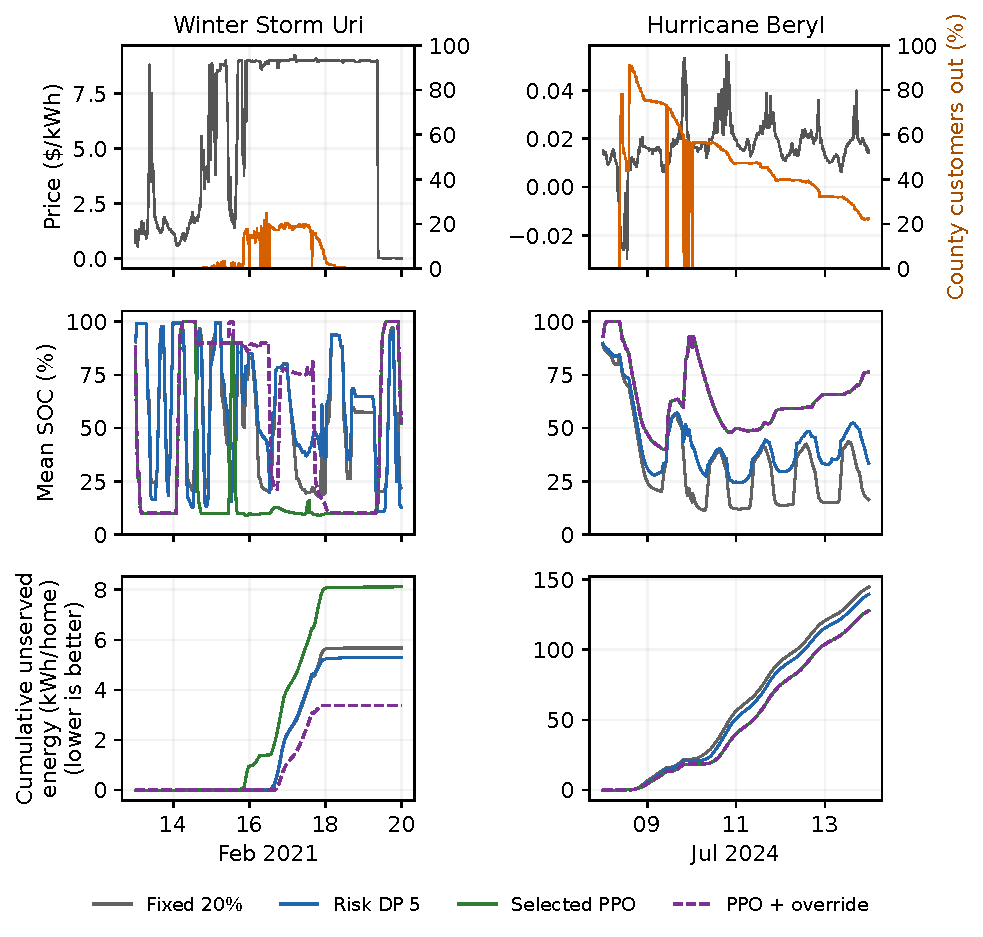
\includegraphics[width=\linewidth]{figs/event_traces.pdf}
\caption{Houston storm traces under identical sampled homes and outages. Top: observed price (gray, left axis) and recorded county outage fraction (orange, right axis). Middle: average fleet SOC, which can conceal individual depleted homes. Bottom: cumulative unserved energy per sampled home, lower is preferable. Full-outage unserved energy can continue rising after a five-hour commitment has already succeeded. Time is local.}
\label{fig:traces}
\end{figure}

\begin{table}[htbp]
\centering\small
\begin{tabular}{llrrrr}
\toprule
Window & Controller & Margin/wk & Promise (\%) & Unserved & Episodes \\
\midrule
HOU: Uri & Fixed 20\% & -865.1 & 90.9 & 5.7 & 198 \\
HOU: Uri & Storm rule & -783.8 & 100.0 & 2.1 & 198 \\
HOU: Uri & Risk DP 5 & -845.4 & 94.4 & 5.3 & 198 \\
HOU: Uri & Selected PPO & -908.6 & 69.7 & 8.1 & 198 \\
HOU: Uri & PPO + override & -785.4 & 98.0 & 3.4 & 198 \\
HOU: Elliott & Fixed 20\% & 81.1 & 100.0 & 0.0 & 1 \\
HOU: Elliott & Storm rule & 5.1 & 100.0 & 0.0 & 1 \\
HOU: Elliott & Risk DP 5 & 85.8 & 100.0 & 0.0 & 1 \\
HOU: Elliott & Selected PPO & 12.5 & 100.0 & 0.0 & 1 \\
HOU: Elliott & PPO + override & 22.2 & 100.0 & 0.0 & 1 \\
HOU: Derecho & Fixed 20\% & 11.0 & 87.6 & 5.6 & 89 \\
HOU: Derecho & Storm rule & 10.9 & 87.6 & 5.5 & 89 \\
HOU: Derecho & Risk DP 5 & 10.0 & 92.1 & 5.2 & 89 \\
HOU: Derecho & Selected PPO & 6.7 & 96.6 & 4.2 & 89 \\
HOU: Derecho & PPO + override & 6.7 & 96.6 & 4.2 & 89 \\
HOU: Beryl & Fixed 20\% & 7.8 & 81.6 & 144.5 & 261 \\
HOU: Beryl & Storm rule & 7.8 & 83.1 & 141.5 & 261 \\
HOU: Beryl & Risk DP 5 & 7.3 & 96.9 & 139.3 & 261 \\
HOU: Beryl & Selected PPO & 7.0 & 97.7 & 127.8 & 261 \\
HOU: Beryl & PPO + override & 7.0 & 97.7 & 127.8 & 261 \\
DFW: Elliott & Fixed 20\% & 78.7 & 100.0 & 0.0 & 3 \\
DFW: Elliott & Storm rule & 78.7 & 100.0 & 0.0 & 3 \\
DFW: Elliott & Risk DP 5 & 84.8 & 100.0 & 0.0 & 3 \\
DFW: Elliott & Selected PPO & -3.3 & 100.0 & 0.0 & 3 \\
DFW: Elliott & PPO + override & -3.3 & 100.0 & 0.0 & 3 \\
\bottomrule
\end{tabular}

\caption{Named-window results. Margin is terminal-adjusted \$/home-week, promise is a percentage, and unserved energy is kWh/home over the actual window. Episode counts refer to simulated household episodes and remain common across controllers. An unavailable promise means no scored episode. Higher margin/promise and lower unserved energy are preferable.}
\label{tab:events}
\end{table}

\begin{table}[htbp]
\centering\small
\begin{tabular}{lrrrr}
\toprule
Threshold\% & Events & Active\% & Past 24 h\% & Lead $\ge4$ h\% \\
\midrule
1 & 455 & 35.8 & 47.9 & 2.9 \\
5 & 41 & 85.4 & 97.6 & 19.5 \\
\bottomrule
\end{tabular}

\caption{County warning coverage, all six evaluated counties, 2019--2025. Threshold is the customers-out percentage defining an audit event. ``Active'' means at onset; ``past 24 h'' means any recent qualifying warning and does not require continuity. The last column requires continuous active lead of at least four hours, the worst preset's charging time from its physical minimum. These fractions are not household service-success probabilities.}
\label{tab:alerts}
\end{table}

The synthetic design crosses three prices (50, 1,000, 5,000 \$/MWh), three outage durations (2, 8, 24 h), four warning leads (0, 1, 3, 6 h), and two initial SOC values (10\%, 90\%), giving 72 cases. Six false/missed-warning cases and eight load/SOH/dropout cases give 86 indexed cases in total. One nominal setting repeats as a reference in the robustness block, leaving 85 distinct parameter settings. Each indexed case is evaluated for an always-discharge proposal and selected PPO, both guarded and unguarded, giving 344 comparisons. Thirty-two homes use 25 kWh presets, demand is 2 kW before an optional twofold uplift, and synthetic outages affect a county fraction of 0.5. SOH sensitivity is 0.85 versus one and dropout sensitivity zero versus 0.2. Price remains high through the specified joint-event window; the full episode lasts 48 hours. These controlled perturbations are stress scenarios, not samples from a calibrated event generator.
\FloatBarrier

\section{Risk-forecast diagnostics}
\label{app:hazard}

\begin{table}[htbp]
\centering\small
\begin{tabular}{lrrrrr}
\toprule
Year & Horizon (h) & ROC AUC & Avg. precision & Brier & Positive\% \\
\midrule
2021 & 1 & 0.952 & 0.744 & 0.0114 & 2.50 \\
2021 & 6 & 0.842 & 0.443 & 0.0307 & 4.27 \\
2021 & 24 & 0.728 & 0.357 & 0.0767 & 9.73 \\
2024 & 1 & 0.963 & 0.815 & 0.0083 & 2.49 \\
2024 & 6 & 0.876 & 0.599 & 0.0225 & 4.00 \\
2024 & 24 & 0.774 & 0.415 & 0.0648 & 8.75 \\
2025 & 1 & 0.865 & 0.399 & 0.0072 & 1.02 \\
2025 & 6 & 0.758 & 0.228 & 0.0227 & 2.68 \\
2025 & 24 & 0.678 & 0.204 & 0.0702 & 8.06 \\
\bottomrule
\end{tabular}

\caption{Out-of-training-period county classifier diagnostics pooled across the twelve weather-covered Texas counties used to fit/evaluate the forecast. Larger ROC AUC/average precision and smaller Brier score are preferable. Positive prevalence differs by year/horizon. Evaluation fleets use six of these counties. Calibration on 2020 does not imply calibration under later distribution changes.}
\label{tab:hazard}
\end{table}

Each horizon classifier uses 300 histogram gradient-boosting iterations, learning rate 0.05, at most 31 leaves, balanced class weights, and seed zero. Isotonic calibration is fitted separately at each horizon. Calendar-year membership selects feature timestamps; future-window training labels can extend by at most 24 hours into the next calendar year. This boundary convention is shared by the saved forecast build and remains well before Uri for 2020 calibration. The bundle release freezes the resulting forecast arrays and fitted model.
\FloatBarrier

\section{Fleet sensitivities and runtime}
\label{app:structure}

\begin{table}[htbp]
\centering\small
\begin{tabular}{llrrr}
\toprule
Scenario & Dispatch & $\Delta$ margin/wk & Promise\% & Episodes \\
\midrule
base 100 & fixed20 & +0.0 & 85.9 & 608 \\
base 100 & storm & +7.2 & 89.8 & 608 \\
base 100 & risk5 & +3.3 & 94.9 & 608 \\
size 500 & fixed20 & +0.0 & 84.5 & 2966 \\
size 500 & storm & +11.5 & 88.7 & 2966 \\
size 500 & risk5 & +4.1 & 94.5 & 2966 \\
size 1000 & fixed20 & +0.0 & 84.4 & 5925 \\
size 1000 & storm & +10.4 & 88.5 & 5925 \\
size 1000 & risk5 & +4.5 & 94.0 & 5925 \\
core 70pct & fixed20 & +0.0 & 88.7 & 608 \\
core 70pct & storm & +6.4 & 92.1 & 608 \\
core 70pct & risk5 & +2.1 & 96.5 & 608 \\
dropout 20pct & fixed20 & +0.0 & 86.2 & 608 \\
dropout 20pct & storm & +14.9 & 89.8 & 608 \\
dropout 20pct & risk5 & +1.5 & 94.1 & 608 \\
base 100 & ppo & -14.3 & 88.0 & 608 \\
base 100 & ppo guard & +10.7 & 97.2 & 608 \\
size 500 & ppo & -5.8 & 87.8 & 2966 \\
size 500 & ppo guard & +13.5 & 97.3 & 2966 \\
size 1000 & ppo & -12.4 & 87.6 & 5925 \\
size 1000 & ppo guard & +12.9 & 97.5 & 5925 \\
core 70pct & ppo & -20.6 & 89.3 & 608 \\
core 70pct & ppo guard & +10.1 & 99.0 & 608 \\
dropout 20pct & ppo & -1.9 & 87.8 & 608 \\
dropout 20pct & ppo guard & +18.5 & 97.2 & 608 \\
\bottomrule
\end{tabular}

\caption{Six-window fleet sensitivity collection, not annual evaluation. Margin difference is \$/home-week against fixed 20\% under the same scenario and is weighted by duration. Promise pools household episode/failure counts across the six windows. Scenario names specify fleet size, a 70\% Core mix, or 20\% independent per-interval dropout; other settings match the base 100-home scenario. All sampled source pools contain 300 profiles.}
\label{tab:structure}
\end{table}

\begin{table}[htbp]
\centering\small
\begin{tabular}{rlrr}
\toprule
Homes & Dispatch & Mean ms/interval & SD \\
\midrule
100 & fixed20 & 1.80 & 0.02 \\
100 & risk5 & 2.18 & 0.11 \\
100 & ppo & 0.34 & 0.00 \\
100 & ppo guard & 0.35 & 0.02 \\
500 & fixed20 & 8.47 & 0.09 \\
500 & risk5 & 9.79 & 0.14 \\
500 & ppo & 0.40 & 0.01 \\
500 & ppo guard & 0.41 & 0.00 \\
1000 & fixed20 & 16.84 & 0.22 \\
1000 & risk5 & 19.84 & 0.11 \\
1000 & ppo & 0.49 & 0.00 \\
1000 & ppo guard & 0.51 & 0.02 \\
\bottomrule
\end{tabular}

\caption{Mean CPU wall time per interval for complete forecast/decision/simulation loops, excluding episode reset. Three measured one-day repetitions follow a warm-up for each configuration. The CSV records platform, backend, thread count and all repetitions. DP replans hourly with 32 grid points; PPO acts every interval. These are implementation timings, not communication delays or isolated neural-network inference times.}
\label{tab:latency}
\end{table}
\FloatBarrier

\section{Full static feeder audit}
\label{app:ac}

The feeder has 1,581 load elements. A fixed seed selects battery locations at each penetration; profiles cycle over the same 100 homes across controllers. Nonattached locations use the load/PV reference. We solve 96 quarter-hours after one day of battery replay on April 15 (normal), July 8 (Beryl), and August 20 (heat), 2024. Three controls at two penetrations plus three no-battery references yield 21 rows. Original voltage-dependent load models are retained. The voltage mask uses the source-bus graph of enabled lines and transformers; it does not certify conductor continuity or phase energization. Relay, protection, restoration, feeder feedback, and AC dynamics are omitted.

\begin{table}[htbp]
\centering\small
\setlength{\tabcolsep}{4pt}
\begin{tabular}{llrrrrr}
\toprule
Day & Dispatch & Pen.\% & Voltage range & UV\% & OV\% & Line\% \\
\midrule
beryl & Load/PV reference & 0 & [0.812, 1.108] & 5.2 & 9.4 & 3.1 \\
beryl & Fixed 20\% & 30 & [0.773, 1.108] & 14.6 & 22.9 & 24.0 \\
beryl & Risk DP 5 & 30 & [0.812, 1.108] & 15.6 & 19.8 & 25.0 \\
beryl & PPO + override & 30 & [0.812, 1.108] & 12.5 & 21.9 & 28.1 \\
beryl & Fixed 20\% & 100 & [0.793, 1.108] & 22.9 & 32.3 & 28.1 \\
beryl & Risk DP 5 & 100 & [0.813, 1.109] & 24.0 & 35.4 & 29.2 \\
beryl & PPO + override & 100 & [0.814, 1.110] & 19.8 & 30.2 & 36.5 \\
heat & Load/PV reference & 0 & [0.851, 1.084] & 17.7 & 17.7 & 39.6 \\
heat & Fixed 20\% & 30 & [0.791, 1.120] & 26.0 & 27.1 & 57.3 \\
heat & Risk DP 5 & 30 & [0.792, 1.120] & 30.2 & 34.4 & 61.5 \\
heat & PPO + override & 30 & [0.728, 1.134] & 33.3 & 49.0 & 56.2 \\
heat & Fixed 20\% & 100 & [0.000, 1.140] & 95.8 & 27.1 & 62.5 \\
heat & Risk DP 5 & 100 & [0.000, 1.141] & 91.7 & 28.1 & 63.5 \\
heat & PPO + override & 100 & [0.000, 1.137] & 70.8 & 36.5 & 56.2 \\
normal & Load/PV reference & 0 & [0.889, 1.084] & 5.2 & 5.2 & 4.2 \\
normal & Fixed 20\% & 30 & [0.888, 1.084] & 7.3 & 18.8 & 6.2 \\
normal & Risk DP 5 & 30 & [0.847, 1.084] & 9.4 & 18.8 & 8.3 \\
normal & PPO + override & 30 & [0.889, 1.131] & 5.2 & 21.9 & 20.8 \\
normal & Fixed 20\% & 100 & [0.888, 1.084] & 11.5 & 21.9 & 8.3 \\
normal & Risk DP 5 & 100 & [0.847, 1.084] & 11.5 & 29.2 & 11.5 \\
normal & PPO + override & 100 & [0.889, 1.193] & 5.2 & 21.9 & 20.8 \\
\bottomrule
\end{tabular}

\caption{Full AC audit. Penetration is the percent of load locations assigned battery dispatch. Voltage range is across phase nodes at graph-reachable buses and all intervals, using the mask above. UV/OV are percentages of intervals with any retained phase voltage below 0.95/above 1.05 pu; Line is the percentage with any line current above its nominal ampacity. A small minimum is retained even when the snapshot solver reports convergence. Eighteen phase nodes at unreachable buses have zero voltage and are counted separately in the released CSV. The reference's existing violations prevent treating controller changes as a calibrated grid-compliance assessment.}
\label{tab:ac}
\end{table}
\FloatBarrier

\section{Aging sensitivity conventions}
\label{app:aging}

Calendar fade is fixed at 2\% per year, independent of dispatch. The throughput proxy is $f_{\rm ET}=2.71\times10^{-5}$ times charge-plus-discharge energy divided by twice rated capacity. The cycle proxy is $\sum_j f_{\rm CB}d_j^{2.03}n_j$, with $f_{\rm CB}=5.24\times10^{-4}$, normalized SOC range $d_j$, and rainflow full/half-cycle count $n_j$. These coefficients follow \citet{humiston2026degradation} without recalibration to the commercial packs. Throughput and rainflow fades are annualized by observed duration.

BLAST-Lite 1.1.1 uses \texttt{Lfp\_Gr\_SonyMurata3Ah\_Battery}. Each SOC and completed-hour ambient-temperature trace is tiled and truncated to 365 days, avoiding linear scaling of short-window calendar fade while introducing repetition and boundary discontinuities. Ambient temperature proxies cell temperature; thermal management, chemistry differences, aging feedback, and stochastic long-term cycling are unmodeled. These columns describe model sensitivities under fixed dispatch, rather than calibrated pack-lifetime forecasts.

\begin{table}[htbp]
\centering\small
\begin{tabular}{lrrrr}
\toprule
Dispatch & Mean SOC (\%) & ET & Rainflow & BLAST \\
\midrule
fixed20 & 56.6 & 0.54 & 3.05 & 4.40 \\
hold90 & 80.5 & 0.39 & 2.13 & 5.75 \\
storm & 58.3 & 0.55 & 3.10 & 4.49 \\
risk5 & 65.3 & 0.50 & 2.51 & 4.93 \\
ppo & 77.8 & 0.38 & 2.17 & 5.40 \\
ppo guard & 77.8 & 0.38 & 2.18 & 5.40 \\
\bottomrule
\end{tabular}

\caption{Mean across four 20-home window sensitivities (Beryl, derecho, August heat, and regular window w10). ET and rainflow columns are annualized capacity-loss percentages; BLAST repeats each trace to one year. Equal weighting across these windows is a reporting convention, not a representative annual climate mix. Mean SOC is a percentage. Lower predicted fade is preferable within a model; values across model classes are not interchangeable.}
\label{tab:aging}
\end{table}
\FloatBarrier
